%%%%%%%%%%%%%%%%%%
% Based on https://github.com/jdavis/latex-homework-template
%%%%%%%%%%%%%%%%%%

\documentclass{article}

\usepackage{fancyhdr}
\usepackage{extramarks}

\usepackage{amsmath}
\usepackage{amsthm}
\usepackage{amsfonts}

\usepackage{tikz}
\usepackage[plain]{algorithm}
\usepackage{algpseudocode}

\usetikzlibrary{automata,positioning}

\usepackage{wrapfig}

\usepackage{lipsum}

%for urls
\usepackage{hyperref}
\hypersetup{
	colorlinks = true,
	linkcolor = teal,
	anchorcolor = teal,
	citecolor = teal,
	filecolor = teal,
	urlcolor = teal
}

%%%%%% Basic Document Settings %%%%%%%%%

\topmargin=-0.45in
\evensidemargin=0in
\oddsidemargin=0in
\textwidth=6.5in
\textheight=9.0in
\headsep=0.25in

\linespread{1.1}

%%%%%%%%%%%%%%%%%% Homework Details %%%%%%%%%%%%%%%
% University Seal
% Title
% Due date
% University
% Class
% Instructor
% Author
% Author ID 
\newcommand{\hmwkSeal}{images/logo.png}
\newcommand{\hmwkTitle}{Assignment\ \#1}
\newcommand{\hmwkDueDate}{March 27, 2023}
\newcommand{\hmwkClass}{Neural Networks \& Representation Learning (CS-587)}
\newcommand{\hmwkClassInstructor}{Ass. Prof. N. Komontakis}
\newcommand{\hmwkUniversity}{University of Crete \\Department of Computer Science}
\newcommand{\hmwkAuthorName}{Nikolaos Kougioulis}
\newcommand{\hmwkAuthorID}{ID 1285}


%fancyhdr
\pagestyle{fancy}
\lhead{\hmwkAuthorName\ (\hmwkAuthorID)} %left head
%\chead{\hmwkClass\ \hmwkTitle} %center head
%\rhead{\date{\today}} %right head
\rhead{\hmwkTitle} 
\lfoot{\lastxmark}
\cfoot{\thepage}

\renewcommand\headrulewidth{0.4pt}

% Create Problem Sections %

\newcommand{\enterProblemHeader}[1]{
	\nobreak\extramarks{}{Problem \arabic{#1} continued on next page\ldots}\nobreak{}
	\nobreak\extramarks{Problem \arabic{#1} (continued)}{Problem \arabic{#1} continued on next page\ldots}\nobreak{}
}

\newcommand{\exitProblemHeader}[1]{
	\nobreak\extramarks{Problem \arabic{#1} (continued)}{Problem \arabic{#1} continued on next page\ldots}\nobreak{}
	\stepcounter{#1}
	\nobreak\extramarks{Problem \arabic{#1}}{}\nobreak{}
}

\setcounter{secnumdepth}{0}
\newcounter{partCounter}
\newcounter{exerciseCounter}
\setcounter{exerciseCounter}{1}
\nobreak\extramarks{Problem \arabic{exerciseCounter}}{}\nobreak{}

% Homework Problem Environment %
% This environment takes an optional argument. When given, it will adjust the problem counter. This is useful for when the problems given for your
% assignment aren't sequential. See the last 3 problems of this template for an example.
%

\newcommand{\enterExerciseHeader}[1]{
	\nobreak\extramarks{}{Exercise \arabic{#1} continued on next page\ldots}\nobreak{}
	\nobreak\extramarks{Exercise \arabic{#1} (continued)}{Exercise \arabic{#1} continued on next page\ldots}\nobreak{}
}

\newcommand{\exitExerciseHeader}[1]{
	\nobreak\extramarks{Exercise \arabic{#1} (continued)}{Exercise \arabic{#1} continued on next page\ldots}\nobreak{}
	\stepcounter{#1}
	\nobreak\extramarks{Exercise \arabic{#1}}{}\nobreak{}
}

\newenvironment{Exercise}[1][-1]{
	\ifnum#1>0
	\setcounter{exerciseCounter}{#1}
	\fi
	\section{Exercise \arabic{exerciseCounter}}
	\setcounter{partCounter}{1}
	\enterExerciseHeader{exerciseCounter}
}{
	\exitExerciseHeader{exerciseCounter}
}



% Title Page %
\title{
	\centering
	\includegraphics[height=1.5in]{\hmwkSeal}
	
	\vspace{1in}
	\textmd{\textbf{\hmwkClass\ \hmwkTitle}}\\
	
	\normalsize\vspace{0.1in}\small{Due\ on\ \hmwkDueDate}\\
	
	\vspace{0.1in}
	\large{\textit{\hmwkClassInstructor}} \\
	\vspace{0.5in}
	
	\large{\hmwkUniversity}
	
	\vspace{3in}
	
	\author{\textbf{\hmwkAuthorName} (\hmwkAuthorID)}
	\date{\today}
}

% Various Helpers %
\newcommand{\alg}[1]{\textsc{\bfseries \footnotesize #1}}
% For derivatives
\newcommand{\deriv}[1]{\frac{\mathrm{d}}{\mathrm{d}x} (#1)}
% For partial derivatives
\newcommand{\pderiv}[2]{\frac{\partial}{\partial #1} (#2)}
% Integral dx
\newcommand{\dx}{\mathrm{d}x}
\newcommand{\E}{\mathbb{E}}
\newcommand{\Var}{\mathrm{Var}}
\newcommand{\Cov}{\mathrm{Cov}}
\newcommand{\Bias}{\mathrm{Bias}}
\newcommand{\Prob}{\mathbb{P}}

\def\code#1{\texttt{#1}}

%for code listings
\usepackage{listings}
\usepackage{xcolor}

\definecolor{codegreen}{rgb}{0,0.6,0}
\definecolor{codegray}{rgb}{0.5,0.5,0.5}
\definecolor{codepurple}{rgb}{0.58,0,0.82}
\definecolor{backcolour}{rgb}{0.99,0.99,0.99}

\lstdefinestyle{mystyle}{
	backgroundcolor=\color{backcolour},   
	commentstyle=\color{codegreen},
	keywordstyle=\color{magenta},
	numberstyle=\tiny\color{codegray},
	stringstyle=\color{codepurple},
	basicstyle=\ttfamily\footnotesize,
	breakatwhitespace=false,         
	breaklines=true,                 
	captionpos=b,                    
	keepspaces=true,                 
	numbers=left,                    
	numbersep=5pt,                  
	showspaces=false,                
	showstringspaces=false,
	showtabs=false,                  
	tabsize=2
}

\lstset{style=mystyle}

\begin{document}
	
	\maketitle
	
	\pagebreak
	
	\subsection{Assignment 1}
    
    %\textbf{Solution} \\
    
    In this assignment we are asked to implement a linear parametric model using Stochastic Gradient Descent (SGD), by using the mini-batch SGD algorithm on the well-examined CIFAR-10 dataset in order to train a linear classifier of the form 
    
    $$f(x;W,b) \equiv Wx + b $$
    
    where $W \in \mathbb{R}^{10 \times D}$ is the weight matrix, $b$ a $10 \times 1$ bias vector, and $x$ a vectorized image $ \in \mathbb{R}^{D \times 1}$, for a total of $C=10$ classes (image categories). \\
    
    \begin{figure}[t]
    	\centering
    	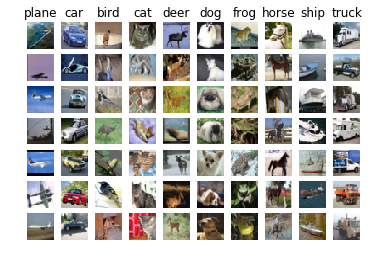
\includegraphics[width=8cm]{images/cifar10.png}
    	\caption{Illustration of the CIFAR-10 dataset.  CIFAR-10 consists of 50,000 training images, belonging in one of ten categories. The task is an image classification problem.}
    \end{figure}

    In order to train our classifier, we have to minimize the regularized empirical loss function
    
    $$\mathcal{L}(W,b) = \frac{1}{N} \sum_{i=1}^{N} \text{Loss}(f(x_i;W,b),y_i) + \lambda R(W)$$
    
    where $\text{Loss}$ is the hinge-loss function $\displaystyle \text{Loss}(s,y) = \text{max}(0, 1 + \text{max}_{j \neq y}s_j - s_y)$ \\

    where $\lambda \in \mathbb{R}$ is the regularization strength and the regularizing norm $R_2(W)$ is either the $L^2$  regularizing norm $\displaystyle R(W) = \sum_{i,j} W_{i,j}^2$ or the $L^1$ regularizing norm $\displaystyle R_1(W) = \sum_{i,j} W_{i,j}$.
    
    To train the classifier using mini-batch SGD, we randomly sample (preferably with replacement, a technique known as \textit{bootstrapping}, otherwise \textit{jacknifing}) a mini-batch of size $M << N$ , consisting of $M$ training data $\left\{ (x_i, y_i)\right\}_{i}$ where $x_i$ are input vectors and $y_i$ their respective ground truth class (true label). We then seek to solve the optimization problem of minimizing the mini-batch loss 
    
    $$\mathcal{L}_{\text{SGD}}(W,b) = \frac{1}{M} \sum_{i=1}^{M} \text{Loss}(f(x_i;W,b),y_i) + \lambda R(W)$$
      
    and update each parameter $\theta$ of the model as $\theta_{\text{new}} \leftarrow \theta_{\text{old}} - \gamma \cdot \frac{\partial L_\text{SGD}}{\partial \theta} $. Hence, for our parameters
    
    $$\displaystyle W \leftarrow W - \gamma \cdot \left( \frac{\sum_{i=1}^{M} \nabla_W \text{Loss}(f(x_i;W,b),y_i)}{M} + \lambda \nabla_W R(W) \right) $$
    
    $$\displaystyle b \leftarrow b - \gamma \left( \cdot \frac{\sum_{i=1}^{M} \nabla_W \text{Loss}(f(x_i;W,b),y_i)}{M} \right) $$
    
    It is unavoidable having to compute the gradient of our loss function (or in intractable cases by using numerical analysis techniques like Euler's method) which for a single point is 
   
    $$\displaystyle L_i = max [\ 0, max_{j \neq y_i}w_j x_i - w_{y_i}x_i + 1\ ]$$
    
    where $x$ is a vectorized image $\in \mathbb{R}^{D \times 1}$, $w_j$ are row vectors, $j$ iterates over the $C=10$ classes, $i$ over all examples and $y_i$ is the index of the ground truth class of $x_i$. The above loss function is known as the Crammer-Singer hinge loss function. 
    
    %The equivalent Weston-Watkins hinge loss function is also used\footnote{\url{https://en.wikipedia.org/wiki/Hinge\textunderscore loss}}, summing over all $j \neq y_i$ instead of two nested max functions, $L_i = \sum\limits_{j \neq y_i}[\ max(0, w_jx_i - w_{y_i}x_i + 1)\ ]$. 
    
    
    The gradient we are looking to compute analytically is $ \nabla_{w_{j}}Li$, which is
    
    $$ \nabla_{w_{j}}Li =  L_i \begin{bmatrix}
    	\frac{\theta Li}{\theta w_{j1}} \\[10pt]
    	\frac{\theta Li}{\theta w_{j2}} \\[10pt]
    	\vdots \\
    	\frac{\theta Li}{\theta w_{jD}}
    \end{bmatrix}
    $$
    
    for all $i= 1,2,\ldots,N$ and  $j=1,\ldots C$.
    
    Notice that for all $k=1,2,\ldots,C$ except the ground truth $y_i$, 
    
    $$\frac{\theta Li}{\theta w_{kj}} = (\mathbf{1}(w_k x_i +1 > 0) +1) x_{ij} - w_{y_i}x_i$$
    
    and for the ground truth $y_i = k$,
    
    $$\frac{\theta Li}{\theta w_{y_i, j}} = -( \mathbf{1}(w_k x_i +1 > 0) + 1) x_{ij} - w_{y_i}x_i$$
    
    where $\mathbf{1}(:)$ denotes the indicator function.
   
    For the derivatives of the regularization terms, we have $\frac{dR_1(W)}{dw} = \text{sign}|W|$ and $\frac{dR_2(W)}{dw} = 2 \sum_{i,j} W$
    
    %Similarly, we can obtain the partials for the equivalent Weston-Watkins hinge loss function,
   
    %$$\frac{\theta Li}{\theta w_{kj}} = \displaystyle  \sum_{j \neq y_i} - \mathbf{1}(w_j x_i - w_{y_i} x_i + 1 > 0) x_i$$
    
    %and 
    %$$\displaystyle \frac{\theta Li}{\theta w_{y_i, j}} = \mathbf{1}(w_jx_i - w_{y_i}x_i + 1 > 0) x_i$$
    
    %for the ground truth $y_i = k$. Both equivalent implementations were tested and they yield same results and select the optimal hyper-parameters (plus-minus the variability of the mini-batch SGD and random sampling with replacement).
    
    \newpage
    

    \vspace{10em}
    
    After filling-in the method \code{compute\textunderscore gradient\textunderscore and\textunderscore loss} that computes the loss and the gradient of the loss on the given training samples and calling that function in \code{train\textunderscore linear\textunderscore classifier} of the \code{LinearClassifier} class, we implement the Stochastic Gradient Descent algorithm in \code{train\textunderscore linear\textunderscore classifier}, execute it on the respective code block of the notebook and plot the loss during training. The resulting loss function plot is shown in Figure 2. \\
    
     \begin{figure}[t]
    	\centering
    	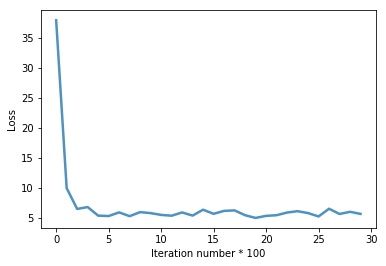
\includegraphics[width=8cm]{images/loss.png}
    	\caption{Training loss during training of the mini-batch SGD, with learning rate = $e^{-7}$, regularization strength $= 5 e^4$, $L^2$ regularization norm, 6 epochs, batch size $= 100$ and number of validation loss intervals $= 100$. Notice the sudden drop at the first number of iterations and the spikes after the first few hundred iterations. The oscillations are a direct consequence of mini-Batch Gradient Descent, as for some mini-batches, during sampling, unfavorable samples have been selected for the optimization.}
    \end{figure}
    
    To predict the most favorable image class, we choose the one with the highest score using \code{np.argmax}. After running the code block to evaluate the performance of the linear classifier on both the training and validation set, we obtain a training accuracy of \code{0.343} and validation accuracy of \code{0.363}. \\
    
    We then proceed to perform hyper-parameter tuning (selecting the optimal value of the hyper-parameters), to obtain the optimal model by testing different values for the learning rate, regularization type, regularization strength and mini-batch size, by training 8 different classifiers to such combinations (one combination per column) on the training set and selecting the one that achieves the highest accuracy on the validation set. \\

    When searching for the optimal hyper-parameters such as learning rate and regularization strength, it is advisable to perform search on log scale. For instance, sampling for a learning rate using $\displaystyle e^{\mathcal{U}(-5,-1)}$ where $\mathcal{U}(a,b)$ is the discrete uniform distribution, as both the learning rate $\gamma$ and the regularization strength multiply the gradient at each update. When choosing the optimal hyper-parameters, as well as when comparing the results of tuning, it is important to note the following: \\
    
    A learning rate that is too small can cause the learning method to get stuck on a local minimum (sub-optimal solution), while a learning rate that is too large can cause the learning method to jump around and converge too quickly to a sub-optimal solution as well. For instance, the model may be close to the optimal solution and all of the sudden end up to a flat plateau. This would make the gradient very close to zero and hence hinder the ability of the model to move out off the plateau to an optimal solution, thus making our model unstable. Regarding the batch size of mini-batch SGD, it's size determines how many examples we would look at before we make a weight update. The lower the batch size, the more noise our training signal is going to have. The higher the batch size, the higher the computational time to compute the gradient at each step. Choosing between the regularization norm is also of high importance: The $L^1$ (lasso norm) tends to shrink coefficients to zero whereas the $L^2$ (ridge) norm tends to shrink coefficients more evenly. It is also significant to note that SGD converges faster than normal stochastic gradient descent since the update of the weights is done after looking at a randomly selected subset of the training set. \\
    
    After performing column-wise hyper-parameter tuning, we obtain the following output for the best classifier based on our combination of hyper-parameters: \\
    
    \code{best training and validation accuracy achieved during cross-validation: 0.373224 and 0.386000
    	using parameters: lr 3.000000e-07 reg 1.000000e+04 reg\textunderscore type 2 and batch\textunderscore size 400}
 
    \vspace{8pt}
    
    Finally, we plot the sequence of mini-batch and validation losses during training of the optimal classifier (Figure 3). By evaluating the classifier on the test set, we obtain an accuracy of \code{0.375}. \\
    
    \begin{figure}[t]
    	\centering
    	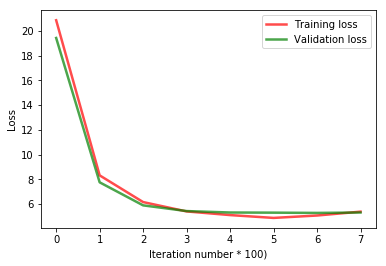
\includegraphics[width=8cm]{images/training_vs_validation_loss.png}
    	\caption{Plot of the training loss and validation loss for every hundred iterations of the optimal model. Note that after the first hundred number of iterations, validation loss becomes higher than training loss.}
    \end{figure}
   
    
    As a final step, it is important to visualize the weights W. Notice in Figure 4, how the weights appear blurry, and, at first glance, resemble visual properties of the examples in each class. For instance, most frogs in CIFAR-10 belong to a species where green is the dominant hue, hence the green color in the middle of the weight matrix for the \code{frog} class. Also notice an example of teratogenesis in the matrix of the horse class, where a brown horse appears to be two-headed (both the color and the two heads are interpreted by the attempt of the model to fit training examples of horses directed to the left or right, primarily brown in color. Some remarks regarding the CIFAR-10 dataset are the following, that fully explain our previous remarks. \\
   
    \begin{figure}[t]
    	\centering
    	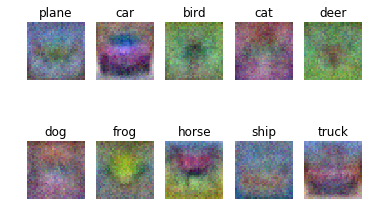
\includegraphics[height=5cm]{images/weights.png}
    	\caption{Visualization of the weights W. The weight matrix for each class appears blurry, as the model attempts to keep a low generalization loss, while all weight matrices depict the main visual characteristics of each training example, to keep a low training loss. For the ship class, blue is dominant as the majority of training images belonging to the ship class are taking at the sea, green is dominant for images of deer because they are wild animals, most training images in the car class were taken with the car facing the camera etc.}
    \end{figure}
    
    
    \begin{enumerate}
    	\item The objects within classes in this dataset can be extremely varied. To name a few, the car class contains family cars, sports cars, racecars and more, all at different angles and poses. For other classes such as horse, our example images appear in different kinds of lighting, environment, some contain the complete body of the animal, others only parts like the head etc. 
    	\item The CIFAR-10 dataset is not large enough to adequately contain examples of everything that is asked for in the test set. This may arise if the training set does not include enough diverse examples. If a rare species of frog is present in the test set and not in the training set, the model will not be able to correctly identify the frog in the test set.
    \end{enumerate}

\begin{thebibliography}{4}
	\bibitem{goodfellow2016} Goodfellow, I., Bengio, Y., \& Courville, A. (2016). \textit{Deep learning}. MIT Press.
	\bibitem{bengio2012} Bengio, Y. (2012). \textit{Practical recommendations for gradient-based training of deep architectures}. Neural Networks: Tricks of the Trade: Second Edition, 437-478.
	\bibitem{zhang2014} Li, M., Zhang, T., Chen, Y., \& Smola, A. J. (2014, August). \textit{Efficient mini-batch training for stochastic optimization}. In Proceedings of the 20th ACM SIGKDD international conference on Knowledge discovery and data mining (pp. 661-670).
	\bibitem{efron1982} Efron, B. (1982). \textit{The jackknife, the bootstrap, and other resampling plans}. Philadelphia, PA: Society for Industrial and Applied Mathematics.
\end{thebibliography}

\end{document}
